\documentclass[tikz,border=5pt]{standalone}
\usepackage{amsmath}
\usepackage{amsfonts}
\usetikzlibrary{shapes.geometric, arrows.meta, positioning, fit, backgrounds, calc}

\begin{document}
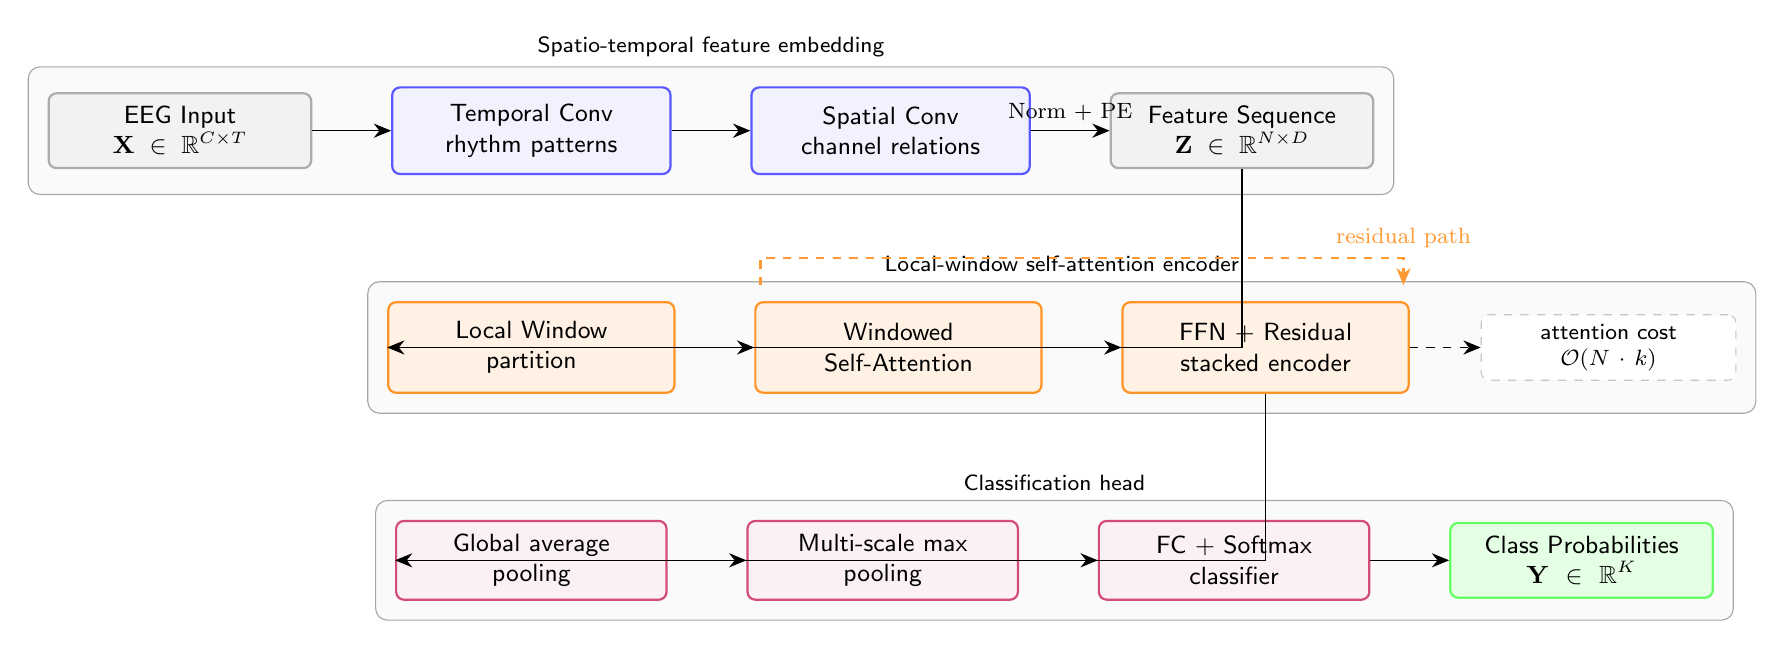
\begin{tikzpicture}[
    font=\sffamily\small,
    >={Stealth[length=2.2mm, width=1.8mm]},
    data/.style={
        rectangle,
        draw=gray!65,
        fill=gray!10,
        thick,
        text width=3.1cm,
        align=center,
        rounded corners=1mm,
        minimum height=0.95cm
    },
    block/.style={
        rectangle,
        draw=blue!65,
        fill=blue!5,
        thick,
        text width=3.3cm,
        align=center,
        rounded corners=1mm,
        minimum height=1.1cm
    },
    attn/.style={
        rectangle,
        draw=orange!85,
        fill=orange!10,
        thick,
        text width=3.4cm,
        align=center,
        rounded corners=1mm,
        minimum height=1.15cm
    },
    head/.style={
        rectangle,
        draw=purple!70,
        fill=purple!6,
        thick,
        text width=3.2cm,
        align=center,
        rounded corners=1mm,
        minimum height=1.0cm
    },
    note/.style={
        rectangle,
        draw=gray!45,
        fill=white,
        dashed,
        text width=3.0cm,
        align=center,
        rounded corners=1mm,
        minimum height=0.75cm,
        font=\sffamily\footnotesize
    },
    group/.style={
        draw=black!35,
        fill=black!2,
        rounded corners=1.5mm,
        inner sep=7pt
    }
]

% Top row: feature embedding
\node[data] (input) {EEG Input\\$\mathbf{X}\in\mathbb{R}^{C\times T}$};
\node[block, right=1.0cm of input] (tconv) {Temporal Conv\\rhythm patterns};
\node[block, right=1.0cm of tconv] (sconv) {Spatial Conv\\channel relations};
\node[data, right=1.0cm of sconv] (seq) {Feature Sequence\\$\mathbf{Z}\in\mathbb{R}^{N\times D}$};

\draw[->] (input) -- (tconv);
\draw[->] (tconv) -- (sconv);
\draw[->] (sconv) -- node[above, font=\footnotesize] {Norm + PE} (seq);

\begin{scope}[on background layer]
    \node[group, fit=(input)(tconv)(sconv)(seq), label={[font=\sffamily\footnotesize]above:Spatio-temporal feature embedding}] {};
\end{scope}

% Middle row: local attention encoder
\node[attn, below=1.6cm of tconv] (win) {Local Window\\partition};
\node[attn, right=1.0cm of win] (attn) {Windowed\\Self-Attention};
\node[attn, right=1.0cm of attn] (ffn) {FFN + Residual\\stacked encoder};
\node[note, right=0.9cm of ffn] (complexity) {attention cost\\$\mathcal{O}(N\cdot k)$};

\draw[->] (seq.south) |- (win.west);
\draw[->] (win) -- (attn);
\draw[->] (attn) -- (ffn);
\draw[->, dashed, orange!80, thick] ($(attn.north west)+(0.08,0.20)$) -- ++(0,0.35) -| ($(ffn.north east)+(-0.08,0.20)$)
    node[midway, above, font=\footnotesize] {residual path};
\draw[->, dashed] (ffn) -- (complexity);

\begin{scope}[on background layer]
    \node[group, fit=(win)(attn)(ffn)(complexity), label={[font=\sffamily\footnotesize]above:Local-window self-attention encoder}] {};
\end{scope}

% Bottom row: classification head
\node[head, below=1.6cm of win] (gap) {Global average\\pooling};
\node[head, right=1.0cm of gap] (msp) {Multi-scale max\\pooling};
\node[head, right=1.0cm of msp] (fc) {FC + Softmax\\classifier};
\node[data, right=1.0cm of fc, draw=green!60, fill=green!10] (output) {Class Probabilities\\$\mathbf{Y}\in\mathbb{R}^{K}$};

\draw[->] (ffn.south) |- (gap.west);
\draw[->] (gap) -- (msp);
\draw[->] (msp) -- (fc);
\draw[->] (fc) -- (output);

\begin{scope}[on background layer]
    \node[group, fit=(gap)(msp)(fc)(output), label={[font=\sffamily\footnotesize]above:Classification head}] {};
\end{scope}

\end{tikzpicture}
\end{document}
